\cleardoublepage

\section{预备知识}
在本节,我们将给出一些符号和定义。在之后的部分,我们会直接使用这些符号和结论。
\subsection{基础符号}
首先定义计算域$[a,b]$的一个剖分
\begin{align*}
    I_{j} = (x_{j-1/2}, x_{j+1/2}), \ j = 1, 2, ..., N
\end{align*}
其中$a=x_{1/2} < x_{3/2}< ...< x_{N+1/2}=b$,N表示网格数。接着定义
\begin{align*}
    \Delta x_j = x_{j+1/2}-x_{j-1/2}, \quad h = \max{\sup_j{\Delta x_j}}, \quad x_j = (x_{j+1/2}+x_{j-1/2})/{2},
\end{align*}
其中$\Delta x_j$表示网格大小,$h$表示网格长度,$x_j$表示网格中点。

网格上有限维计算空间$V_h^k = \{v:v|_{I_j}\in P^k(I_j); 1\leq j\leq N\}$,其中$P^k(I_j)$表示$I_j$上次数不大于$k$的多项式集合。我们的数值解和测试函数都将从$V_h^k$中取得。需要注意的是,$V_h^k$中的函数在单元边界节点处不一定是连续的,可以出现跳跃。

为了简化标记,我们分别定义$(u_h)^+_{j+1/2}=u_h(x^+_{j+1/2})$和$(u_h)^-_{j+1/2}=u_h(x^-_{j+1/2})$。此外我们定义$u_h$在单元边界节点$x_{j+1/2}$的跳跃$[u_h]_{j+1/2}=(u_h)^+_{j+1/2}-(u_h)^-_{j+1/2}$和均值$(\overline{u}_h)_{j+1/2}=((u_h)_{j+1/2}^++(u_h)_{j+1/2}^-)/2$。

\subsection{间断伽辽金方法基本理论}

我们有以下事实\cite{sullivan2020brief}:
\begin{itemize}
    \item 许多PDEs没有强解但有弱解
    \item 弱解更容易在线性代数表示
    \item 即使强解存在,证明弱解存在性再说明其具有强解的性质往往比直接找到一个强解要简单
\end{itemize}
而我们的DD模型的强解很难求出,因此我们期望弱化要求,求得一个对于测试函数满足我们真正关心的性质的弱解,这同时也能给我们带来编程上的简便。

为了得到这样的弱解,我们想法是在方程两边乘上测试函数并积分得到弱形式,利用数值方法求解弱形式。以
\begin{align}
    u_t + f_x = 0\label{eq:SDG}
\end{align}
为例,我们在\eqref{eq:SDG}两边乘以测试函数v并积分整理得到
\begin{equation}
    \int_{I_i}u_t v_h\mathrm{d}x - \int_{I_i}f(u)(v_h)_x\mathrm{d}x+v_hf\bigg|^{x_{i+\frac{1}{2}}}_{x_{i-\frac{1}{2}}}.
\end{equation}
这里f需要用的隔壁单元的值,为了处理这一问题,需要采用数值通量
\begin{equation*}
    \hat{f}_{i+\frac{1}{2}}=\hat{f}(u_h(x^-_{i+\frac{1}{2}},t),u_h(x^+_{i+\frac{1}{2}},t))
\end{equation*}
来代替f。具体来说,数值通量$\hat{f}$需要满足下列要求:
\begin{enumerate}
    \item 一致性:$\hat{f}(u,u)=f(u)$。
    \item 连续性:$\hat{f}$关于两个变量都是Lipschitz连续的。
    \item 单调性:$\hat{f}$关于第一个变量单增,关于第二个单减。可以记作$\hat{f}(\uparrow,\downarrow)$。
\end{enumerate}
这些性质将保证间断伽辽金法(DGM)的稳定性。
现在我们得到弱形式。
\begin{equation}
    \int_{I_i}u_t v_h\mathrm{d}x - \int_{I_i}f(u)(v_h)_x\mathrm{d}x+\hat{f}_{i+\frac{1}{2}}v_h(x^-_{i+\frac{1}{2}})-\hat{f}_{i-\frac{1}{2}}v_h(x^+_{i-\frac{1}{2}}) = 0. \label{DG:weakSolution}
\end{equation}
间断伽辽金法的想法就是找到独一无二的数值解$u_h^k\in V_h^k$使得对于任意的测试函数,弱形式\eqref{DG:weakSolution}都成立。但是对于高阶PDEs,按照上述流程无法整理为形如\eqref{DG:weakSolution}的弱形式,因此我们需要考虑改进DGM来解决这样的PDEs。
\subsubsection{局部间断伽辽金法}
改进的方法有多种,在本文我们采用的是局部间断伽辽金法(LDG)。LDG法的想法是引入一个辅助变量来使得含有高阶偏导的PDE降阶为只含一阶导的PDEs,然后在这些一阶PDEs上应用DG法。
\begin{equation}
    u_t = u_{xx}
\end{equation}
令$v = u_x$得到
\begin{align}
    u_t - v_x = 0, \\
    v - u_x = 0.
\end{align}
现在我们可以利用DGM来处理该高阶PDE了。
\subsubsection{限制器}
当但DG法依然存在数值振荡,特别是对于包含强离散的问题,因此我们使用限制器来限制震荡,同时保证全变差稳定性。限制器的想法是先对当前时间层的数值解进行一个预处理,然后再更新至下一个时间层。本文将采用一种实际中常用的满足全变差有界(TVB)的改进后的minmod限制器\cite{cockburn1989tvb2}。

对于$I_j$上的解$u_h$,首先定义它的平均值
$$
    \overline{u}_j = \frac{1}{\Delta x_j}\int_{I_j}u_h dx,
$$
然后我们定义
\begin{align}
    \tilde{u}_j = m(u_h(x^-_{j+1/2})-\overline{u}_j, \Delta_+\overline{u}_j, \Delta_-\overline{u}_j), \quad \tilde{\tilde{u}}_j = m(\overline{u}_j-u_h(x^+_{j-1/2}), \Delta_+\overline{u}_j, \Delta_-\overline{u}_j),
\end{align}
其中$\Delta_+$和$\Delta_-$是差分算子,定义为
\begin{align}
    \Delta_+\overline{u}_j = \overline{u}_{j+1}-\overline{u}_{j}, \quad \Delta_-\overline{u}_j = \overline{u}_{j}-\overline{u}_{j-1},
\end{align}
minmod函数$m$定义为
\begin{align}
    m(a_1, ..., a_l) & =
    \begin{cases}
        a_1,                         & |a_1| \leq M                                              \\
        s \min_{1\leq i\leq l}|a_i|, & |a_1| \leq M \text{且}s = sign(a_1) = \cdots = sign(a_l), \\
        0 ,                          & \text{其他},
    \end{cases}
\end{align}
这里面的TVB参数M选择有多种选择方式,本文采用相对简便的一种\cite{cockburn1989tvb3}
\begin{align}
    M = \frac{2}{3}\max_{\Omega}u_{xx},
\end{align}
其中$\Omega$表示$u$所有驻点的附近的集合。
最后我们有
\begin{align}
    u^{(mod)}_h(x^-_{j+1/2}) = \overline{u}_j + \tilde{u}_j, \quad u^{(mod)}_h(x^+_{j-1/2}) = \overline{u}_j - \tilde{\tilde{u}}_j.
\end{align}
上述限制限制器本质上是在满足单元平均值$\overline{u}_j$不变的前提下重新计算单元边界处的值。最终,我们能够得到单元平均值以及单元边界的值,因此我们可以唯一求出一个$k\leq 2$的多项式。但是对于$k> 2$的情况需要更复杂的分析,简单地把更二次多项式看作更高次多项式可能会导致损失精度。
\subsection{龙格库塔法主要案例}
龙格-库塔法(RK)是一种重要的迭代法。一般的显示龙格-库塔法可以表示为
\begin{equation}
    \begin{aligned}
        u^{(i)} = \sum_{l=0}^{i-1}[\alpha_{i,l}u^{(l)} + \beta_{i,l}\Delta tL(u^{(l)})], \quad i = 1,...,m,
        u^{(0)}=u^n,\quad u^{(m)} = u^{n+1}.
    \end{aligned}
    \label{eq:TVDRK}
\end{equation}

由\parencite{shu1998total},我们有得到
\begin{lemma}
    当$a_{ik} \geq 0, \beta_{ik} \geq 0$时,在时间步长$\Delta t \leq \frac{\beta_{ik}}{\alpha_{ik}} \Delta t_1$的条件下,龙格-库塔法\eqref{eq:TVDRK}满足全变差不增。
\end{lemma}

特别地对于三阶TVD RK法,\parencite{shu1998total}给出了最优形式
\begin{equation}
    \begin{aligned}
        u^{(1)} & = u^n + \Delta t L(u^n),                                                \\
        u^{(2)} & = \frac{1}{2}u^n + \frac{1}{4}u^{(1)} + \frac{1}{4}\Delta L(u^{(1)})),  \\
        u^{n+1} & = \frac{1}{3}u^n + \frac{2}{3}u^{(2)} + \frac{2}{3}\Delta t L(u^{(2)}), \\
        CFL     & = 1.
    \end{aligned}
\end{equation}

对于IMEXRK法,本文考虑三阶精度的四阶段,L-稳定的对角隐式龙格-库塔法(DIRK)耦合四阶段显式龙格-库塔(ERK)法\cite{ascher1997implicitexplicita},它们的Butcher表分别是:
\begin{table}
    \begin{minipage}{0.48\linewidth}
        \centering
        \begin{tabular}{c|cccc}
            $\frac{1}{2}$ & $\frac{1}{2}$  & 0              & 0             & 0             \\
            $\frac{2}{3}$ & $\frac{1}{6}$  & $\frac{1}{2}$  & 0             & 0             \\
            $\frac{1}{2}$ & $-\frac{1}{2}$ & $\frac{1}{2}$  & $\frac{1}{2}$ & 0             \\
            1             & $\frac{3}{2}$  & $-\frac{3}{2}$ & $\frac{1}{2}$ & $\frac{1}{2}$ \\
            \hline
                          & $\frac{3}{2}$  & $-\frac{3}{2}$ & $\frac{1}{2}$ & $\frac{1}{2}$
        \end{tabular}
        \label{tab:DIRK}
    \end{minipage}
    \begin{minipage}{0.48\linewidth}
        \centering
        \begin{tabular}{c|cccc}
            $\frac{1}{2}$ & $\frac{1}{2}$   & 0              & 0             & 0              \\
            $\frac{2}{3}$ & $\frac{11}{18}$ & $\frac{1}{18}$ & 0             & 0              \\
            $\frac{1}{2}$ & $\frac{5}{6}$   & $-\frac{5}{6}$ & $\frac{1}{2}$ & 0              \\
            1             & $\frac{1}{4}$   & $\frac{7}{4}$  & $\frac{3}{4}$ & $-\frac{7}{4}$ \\
            \hline
                          & $\frac{1}{4}$   & $\frac{7}{4}$  & $\frac{3}{4}$ & $-\frac{7}{4}$
        \end{tabular}
        \label{tab:ERK}
    \end{minipage}
    \caption{DIRK耦合ERK得到的三阶IMEX格式。左:DIRK;右:ERK。}
    \label{tab:IMEX3}
\end{table}

\section{DD模型}

本文采用的DD模型表示为
\begin{align}
    n_t - (\mu En)_x = \tau \theta n_{xx}, \label{eq:DD} \\
    \phi_{xx} = \frac{e}{\epsilon}(n - n_d),  \label{eq:poisson}
\end{align}
其中$x\in(0,1)$,第一个电子浓度方程取周期边界条件,第二个电势方程取Dirichlet边界条件:$\phi(0,t) = 0, \phi(1,t) = v_{bias}$。
在系统\eqref{eq:DD}-\eqref{eq:poisson}中,未知量是电子浓度$n$和电势$\phi$。$m_0$表示电子有效质量,k是玻尔兹曼常数,e是电子电荷,$\mu$代表迁移率,$T_0$是晶格温度,$\tau = \frac{m_0 \mu}{e}$是松弛参数,$\theta = \frac{k}{m_0}T_0$,$\epsilon$是介电常量,$n_d$是一个给定的掺杂函数。

\subsection{TVDRK LDG格式}
取$q = \sqrt{\tau \theta }n_x$,那么\autoref{eq:DD}可以写作
\begin{align}
    n_t - (\mu E n)_x - \sqrt{\tau \theta}q_x & = 0, \label{eq:DD:electronConcentration} \\
    q - \sqrt{\tau \theta}n_x                 & = 0. \label{eq:DD:auxiliaryFunction}
\end{align}
而对于泊松方程,本文直接通过积分得到。

令$E = -\phi_x$表示电势,通过引入辅助变量易证$E$具有周期性\cite{liu2010errorc}。
在方程\eqref{eq:DD:electronConcentration}-\eqref{eq:DD:auxiliaryFunction}两边分别乘以测试函数$v,w\in V_h^k$,分部积分得到
\begin{align}
     & \int_{I_{j}} n_{t} v d x+\int_{I_{j}}(\mu E n+\sqrt{\tau \theta} q) v_{x} d x                                                                               \nonumber                                      \\
     & \quad-(\mu E n+\sqrt{\tau \theta} q)_{j+\frac{1}{2}} v_{j+\frac{1}{2}}^{-}+(\mu E n+\sqrt{\tau \theta} q)_{j-\frac{1}{2}} v_{j-\frac{1}{2}}^{+}=0,            \label{eq:LDG:n}                             \\
     & \int_{I_{j}} q w d x+\int_{I_{j}} \sqrt{\tau \theta} n w_{x} d x-\sqrt{\tau \theta} n_{j+\frac{1}{2}} w_{j+\frac{1}{2}}^{-}+\sqrt{\tau \theta} n_{j-\frac{1}{2}} w_{j-\frac{1}{2}}^{+}=0, \label{eq:LDG:q} \\
     & E_{x}=-\frac{e}{\varepsilon}\left(n-n_{d}\right) .
\end{align}
将上述方程中的精确解$n, q$和$E$替换为它们在$V_{h}^{k}$中的数值近似解$n_h, q_h$。由于数值解$n_h$和$q_h$在单元边界上不连续性,将单元边界上的项替换为适当的数值通量,我们得到LDG格式:
\begin{align}
     & \int_{I_{j}}\left(n_h\right)_{t} v d x+\int_{I_{j}}\left(\mu E_h n_h+\sqrt{\tau \theta} q_h\right) v_{x} d x      \nonumber                                                                                                                    \\
     & \quad-\left(\mu \widehat{E_h n_h}+\sqrt{\tau \theta} \hat{q}_{h}\right)_{j+\frac{1}{2}} v_{j+\frac{1}{2}}^{-}+\left(\mu \widehat{E_h n_h}+\sqrt{\tau \theta} \hat{q}_{h}\right)_{j-\frac{1}{2}} v_{j-\frac{1}{2}}^{+}=0, \label{eq:DDLDGn}     \\
     & \int_{I_{j}} q_h w d x+\int_{I_{j}} \sqrt{\tau \theta} n_h w_{x} d x-\sqrt{\tau \theta} \hat{n}_{j+\frac{1}{2}}^{h} w_{j+\frac{1}{2}}^{-}+\sqrt{\tau \theta} \hat{n}_{j-\frac{1}{2}}^{h} w_{j-\frac{1}{2}}^{+}=0,            \label{eq:DDLDGq} \\
     & E_h=\int_{0}^{x}-\frac{e}{\varepsilon}\left(n_h-n_{d}\right) d x+E_{0}-v_{\text {bias }},\label{eq:DDLDGE}
\end{align}
其中,$E_{0}=E_h(0)=\int_{0}^{1}\left(\int_{0}^{x} \frac{e}{\varepsilon}\left(n_h-n_{d}\right) d s\right) d x$。这里的“$\hat{}$”项表示数值通量。$\hat{n}_{h}$和$\hat{q}_{h}$选择交替通量,即$\hat{n}_{h}=\left(n_h\right)^{+}$,$\hat{q}_{h}=\left(q_h\right)^{-}$,$\widehat{E_h n_h}$采用上风通量,即$\widehat{E_h n_h}=\max \left(E_h, 0\right)\left(n_h\right)^{+}+\min \left(E_h, 0\right)\left(n_h\right)^{-}$。

从LDG格式可知,只要有m时间层的信息,我们可以仅从\eqref{eq:DDLDGq}求得辅助变量$q$,进而求得$m+1$时间层的数值解。这种只需要系统中一个方程求得辅助变量,因此我们这种方法为“局部”间断伽辽金法。这也是与过去需要全局系统才能求出$q$的方法的不同之处。

对于时间离散,我们采用三阶全变差不增(TVD)龙格库塔法。
\begin{align}
    u^{(1)} & = u^n + \Delta t L(u^n),                                                \\
    u^{(2)} & = \frac{3}{4}u^n + \frac{1}{4}u^{(1)} + \frac{1}{4}\Delta t L(u^{(1)}), \\
    u^{n+1} & = \frac{1}{3}u^n + \frac{2}{3}u^{(2)} + \frac{2}{3}\Delta t L(u^{(2)}).
\end{align}
该方法保证$TV(u^{n+1})\leq TV(u^n)$,其中$TV(u) = \sum_j |u_{j+1}-u_j|$。
\subsection{IMEX全离散LDG格式}
本小节,我们将考虑LDG空间离散耦合IMEX时间离散格式。这种IMEX时间离散的想法是显式处理二阶非线性对流项和隐式处理线性扩散项,来减弱对两项都使用显式时间离散所要求的严格的时间步长。这样做可以大量节省我们的算力,同时保持无条件稳定性。

与耦合TVDRK时间离散相比,电子浓度方程\eqref{eq:DD}的处理方式不变,而对于泊松方程\eqref{eq:poisson}我们在此处也对它进行空间离散,具体有:
\begin{align}
    E_x & = -\frac{e}{\epsilon}(n-n_d), \label{eq:poisson:1} \\
    E   & = - \phi_x. \label{eq:poisson:2}
\end{align}
在等式\eqref{eq:poisson:1}-\eqref{eq:poisson:2}两边分别乘上测试函数$r,z\in V^k_h$得到
\begin{align}
     & -\int_{I_j}Er_x\rm{d}x + E_{j+\frac{1}{2}}r_{j+\frac{1}{2}}^- - E_{j-\frac{1}{2}}r_{j-\frac{1}{2}}^+ = -\frac{e}{\epsilon}\int_{I_j}(n-n_d)r\rm{d}x,                                       \label{DD:weakform:E} \\
     & \int_{I_j} Ez \rm{d}x - \int_{I_j}\phi z_x \rm{d}x + \phi_{j+\frac{1}{2}}z_{j+\frac{1}{2}}^- - \phi_{j-\frac{1}{2}}z_{j-\frac{1}{2}}^+ = 0, \label{DD:weakform:phi}
\end{align}

并将单元边界的量替换为对应的数值通量,结合\eqref{eq:DDLDGn}-\eqref{eq:DDLDGq}的DD模型的空间离散形式:
\begin{align}
     & \int_{I_{j}}\left(n_h\right)_{t} v d x+\int_{I_{j}}\left(\mu E_h n_h+\sqrt{\tau \theta} q_h\right) v_{x} d x      \nonumber                                                                                                                       \\
     & \quad-\left(\mu \widehat{E_h n_h}+\sqrt{\tau \theta} \hat{q}_{h}\right)_{j+\frac{1}{2}} v_{j+\frac{1}{2}}^{-}+\left(\mu \widehat{E_h n_h}+\sqrt{\tau \theta} \hat{q}_{h}\right)_{j-\frac{1}{2}} v_{j-\frac{1}{2}}^{+}=0, \label{eq:IMEX:DD:n}     \\
     & \int_{I_{j}} q_h w d x+\int_{I_{j}} \sqrt{\tau \theta} n_h w_{x} d x-\sqrt{\tau \theta} \hat{n}_{j+\frac{1}{2}}^{h} w_{j+\frac{1}{2}}^{-}+\sqrt{\tau \theta} \hat{n}_{j-\frac{1}{2}}^{h} w_{j-\frac{1}{2}}^{+}=0,            \label{eq:IMEX:DD:q} \\
     & -\int_{I_j}E_hr_x\rm{d}x + (\hat{E}_h)_{j+\frac{1}{2}}r_{j+\frac{1}{2}}^- - (\hat{E}_h)_{j-\frac{1}{2}}r_{j-\frac{1}{2}}^+ = -\frac{e}{\epsilon}\int_{I_j}(n_h-n_d)r\rm{d}x,                                        \label{eq:IMEX:poisson:1}     \\
     & \int_{I_j} E_hz \rm{d}x - \int_{I_j}\phi_h z_x \rm{d}x + (\hat{\phi}_h)_{j+\frac{1}{2}}z_{j+\frac{1}{2}}^- - (\hat{\phi}_h)_{j-\frac{1}{2}}z_{j-\frac{1}{2}}^+ = 0,\label{eq:IMEX:poisson:2}
\end{align}
其中$j = 1,...,N$,带“$\widehat{\ }$”的项也是数值通量。我们选择通量$\widehat{E_h n_h} = \frac{1}{2}((E_hn_h)^+  + (E_hn_h)^-)$,$\hat{n}_h$和$\hat{q}_h$的交替通量,即
\begin{equation}
    \hat{n}_h = (n_h)^+, \hat{q}_h = (q_h)^- \quad \text{or} \quad \hat{n}_h = (n_h)^-, \hat{q}_h = (q_h)^+, \label{numbericalFlux:n&q}
\end{equation}
对$\hat{\phi}_h$和$\hat{E}_h$选择带边界条件的交替通量,即
\begin{equation}
    \begin{aligned}
        (\hat{\phi}_h)_{\frac{1}{2}} = (\phi_h^-)_{\frac{1}{2}} = 0, (\hat{\phi}_h)_{j-\frac{1}{2}} = (\phi_h^+)_{j-\frac{1}{2}},j = 2,\cdots,N,(\hat{\phi}_h)_{N-\frac{1}{2}} = (\phi_h^+)_{N-\frac{1}{2}} = v_{bias}, \\
        (\hat{E_h})_{\frac{1}{2}} = (E_h^+)_{\frac{1}{2}} + c_0[\phi]_{\frac{1}{2}}, (\hat{E}_h)_{j-\frac{1}{2}} = (E_h^-)_{j-\frac{1}{2}} + c_0[\phi]_{j-\frac{1}{2}},j = 2,\cdots,N+1,
    \end{aligned}\label{numbericalFlux:phi&E}
\end{equation}
或
\begin{equation}
    \begin{aligned}
        (\hat{\phi}_h)_{\frac{1}{2}} = (\phi_h^-)_{\frac{1}{2}} = 0, (\hat{\phi}_h)_{j-\frac{1}{2}} = (\phi_h^-)_{j-\frac{1}{2}},j = 2,\cdots,N,(\hat{\phi}_h)_{N-\frac{1}{2}} = (\phi_h^+)_{N-\frac{1}{2}} = v_{bias}, \\
        (\hat{E_h})_{j - \frac{1}{2}} = (E_h^+)_{j - \frac{1}{2}} + c_0[\phi]_{j-\frac{1}{2}},j = 2,\cdots,N, (\hat{E}_h)_{N+\frac{1}{2}} = (E_h^-)_{N+\frac{1}{2}} + c_0[\phi]_{N+\frac{1}{2}}.
    \end{aligned}\label{numbericalFlux:phi&E alt}
\end{equation}
在数值模拟中我们选择第一种。

将\autoref{tab:IMEX3}对应的三阶IMEX时间离散分别应用到\eqref{eq:IMEX:DD:n}-\eqref{eq:IMEX:DD:q}和\eqref{eq:IMEX:poisson:1}-\eqref{eq:IMEX:poisson:2}中得到三阶IMEXLDG格式:找到$n_h^{m+1}, q_h^{m+1}\in V_h^k$使得
\begin{align}
    (\frac{n_h^{m,1} -n_h^m}{\Delta t},v)_{I_j} & =\frac{1}{2} H_j(E_h^m,n_h^m,v) + \frac{1}{2} H_j^-(q_h^{m,1},v),           \label{eq:IMEX:DD:LDG:1}                       \\
    (\frac{n_h^{m,2} -n_h^m}{\Delta t},v)_{I_j} & = \frac{1}{18} H_j(E_h^m,n_h^m,v) + \frac{1}{18} H_j(E_h^{m,1},n_h^{m,1},v) \nonumber                                      \\
                                                & + \frac{1}{6} H_j^-(q_h^{m,1},v) + \frac{1}{2} H_j^-(q_h^{m,2},v),                                                         \\
    (\frac{n_h^{m,3} -n_h^m}{\Delta t},v)_{I_j} & =\frac{5}{6} H_j(E_h^m,n_h^m,v) -\frac{5}{6} H_j(E_h^{m,1},n_h^{m,1},v) + \frac{1}{2} H_j(E_h^{m,2},n_h^{m,2},v) \nonumber \\
                                                & - \frac{1}{2} H_j^-(q_h^{m,1},v) + \frac{1}{2} H_j^-(q_h^{m,2},v) + \frac{1}{2} H_j^-(q_h^{m,3},v),                        \\
    (\frac{n_h^{m+1} -n_h^m}{\Delta t},v)_{I_j} & = \frac{1}{4} H_j(E_h^m,n_h^m,v) +\frac{7}{4} H_j(E_h^{m,1},n_h^{m,1},v)  \nonumber                                        \\
                                                & + \frac{3}{4} H_j(E_h^{m,2},n_h^{m,2},v) - \frac{7}{4} H_j(E_h^{m,3},n_h^{m,3},v) \nonumber                                \\
                                                & +\frac{3}{2} H_j^-(q_h^{m,1},v) -\frac{3}{2} H_j^-(q_h^{m,2},v) \nonumber                                                  \\
                                                & + \frac{1}{2} H_j^-(q_h^{m,3},v)  + \frac{1}{2} H_j^-(q_h^{m+1},v),                                                        \\
    (q_h^{m,1},w)_{I_j}                         & = H_j^+(n_h^{m,l},w), l = 1,2,3,4, q_h^{m,4} = q_h^{m+1},\label{eq:IMEX:DD:LDG:4}
\end{align}
其中$j = 1,\cdots,N;\quad v,w \in V_h$,
\begin{align}
     & H_j(E_h,n_h,v)    = - (\mu E_h n_h, v_x)_{I_j} + (\mu \hat{E_h n_h})_{j+\frac{1}{2}}v_{j+\frac{1}{2}}^- - (\mu \hat{E_h n_h})_{j-\frac{1}{2}}v_{j-\frac{1}{2}}^+, \label{eq:IMEX:DD:notation:1}                                        \\
     & H_j^{\pm}(u_h,v)  =- \sqrt{\tau \theta}(u_h,v_x)_{I_j} + \sqrt{\tau\theta}(u_h^{\pm})_{j+\frac{1}{2}}v_{j+\frac{1}{2}}^0 - \sqrt{\tau\theta}(u_h^{\pm})_{j-\frac{1}{2}}v_{j-\frac{1}{2}}^+,\quad u = n,q.\label{eq:IMEX:DD:notation:2}
\end{align}

电势方程的LDG格式是:找到$E_h^{m,l},\phi_h^{m,l} \in V_h$,使得
\begin{align}
    -\int_{I_j} E_h^{m,l}r_x \rm{d}x + (\hat{E}_h^{m,l})_{j+\frac{1}{2}}r_{j+\frac{1}{2}}^- - (\hat{E}_h^{m,l})_{j-\frac{1}{2}}r_{j-\frac{1}{2}}^+ = -\frac{e}{\epsilon}\int_{I_j}(n_h^{m,l} - n_d) r\rm{d} x, \label{eq:IMEX:poisson:LDG:1} \\
    \int_{I_j} E_h^{m,l}z \rm{d}x - \int_{I_j} \phi_h^{m,l}z_x \rm{d}x  + (\hat{\phi}_h^{m,l})_{j+\frac{1}{2}}z^-_{j+\frac{1}{2}} - (\hat{\phi}_h^{m,l})_{j-\frac{1}{2}}z_{j-\frac{1}{2}}^+  = 0,\label{eq:IMEX:poisson:LDG:2}
\end{align}
其中$j = 1,\cdots,N; r,z \in V_h$且$l = 0,1,2,3, u^{m,0} = u^m$。

\subsection{误差估计}
对于三阶IMEX LDG格式,我们有以下误差估计\cite{liu2016analysis}:
\begin{theorem}
    令$n^m,q^m$是问题\eqref{eq:LDG:n}-\eqref{eq:LDG:q}和\eqref{DD:weakform:E}-\eqref{DD:weakform:phi}在时间层级m的精确解,它们足够光滑且有有界导数。令$n_h^m,q_h^m$是三阶IMEX LDG格式\eqref{eq:IMEX:DD:LDG:1} -\eqref{eq:IMEX:DD:LDG:4} 。如果有限元空间$V_h^k$是k$(k\geq  0)$阶间断多项式,那么对于足够小的h,存在与h无关正常数C,使得下列误差估计成立
    \begin{equation}
        ||n-n_h||_{L^{\infty}(0,T;L^2)} + ||q - q_h||_{L^2(0,T;L^2)} \leq C(h^{k+1} + (\Delta t)^3)
    \end{equation}
    其中C依赖于最终时间T,k,反常数$C_2$, $||n||_{L^{\infty}(0,T;H^{k+1})}$,$||n_x||_{L^{\infty}}$和$||E||_{L^{\infty}}$。
\end{theorem}
\section{HF模型}
高场模型由以下方程以及带有周期边界条件的Poisson电场方程~\eqref{eq:poisson}表示
\begin{equation}
    n_{t}+J_{x}=0, \quad x \in(0,1) \label{eq:HF}
\end{equation}
其中
$$
    J=J_{h y p}+J_{v i s}
$$

$$
    \begin{gathered}
        J_{h y p}=-\mu n E+\tau \mu\left(\frac{e}{\varepsilon}\right) n(-\mu n E+\omega) \\
        J_{v i s}=-\tau\left(n\left(\theta+2 \mu^{2} E^{2}\right)\right)_{x}+\tau \mu E(\mu n E)_{x} .
    \end{gathered}
$$
这里,$\omega=\left.(\mu n E)\right|_{x=0}$取常数。
\subsection{TVDRK LDG格式}
未知量与DD模型中相同:电子浓度$n$和电势$\phi$。由于
$$
    -2\left(n E^{2}\right)_{x}+E(n E)_{x}=-3 n E E_{x}-E^{2} n_{x}
$$
上述方程可以写作
\begin{equation}
    n_{t}+\left(-\mu n E-\tau \mu^{2} \frac{e}{\varepsilon} n^{2} E+\tau \mu \frac{e}{\varepsilon} \omega n-3 \tau \mu^{2} E n E_{x}\right)_{x}-\left(\left(\tau \theta+\tau \mu^{2} E^{2}\right) n_{x}\right)_{x}=0.\label{eq:HFRewritten}
\end{equation}
利用$E_{x}=-\frac{e}{\varepsilon}\left(n-n_{d}\right)$,定义$C_{1}=\frac{\tau \mu e}{\varepsilon}$,$C_{2}=\frac{\tau \mu^{2} e}{\varepsilon}=\mu C_{1}$和$C_{3}=\frac{\tau \mu e \omega}{\varepsilon}=\omega C_{1}$,方程~\eqref{eq:HFRewritten}可以简写为
\begin{equation}
    n_{t}+\left(-\left(3 C_{2} E n_{d}+\mu E-C_{3}\right) n+2 C_{2} E n^{2}\right)_{x}-\left(\left(\tau \theta+\tau \mu^{2} E^{2}\right) n_{x}\right)_{x}=0 .  \label{eq:HFRewrittenc}
\end{equation}
设$q=\sqrt{\tau \theta+\tau \mu^{2} E^{2}} n_{x}=\left(\sqrt{\tau \theta+\tau \mu^{2} E^{2}} n\right)_{x}-\left(\sqrt{\tau \theta+\tau \mu^{2} E^{2}}\right)_{x} n$,我们可以将方程$~\eqref{eq:HFRewrittenc}$按照LDG的方法改写为更大的一阶PDE系统
\begin{align}
     & n_{t}+\left(-\left(3 C_{2} E n_{d}+\mu E-C_{3}\right) n+2 C_{2} E n^{2}-\sqrt{\tau \theta+\tau \mu^{2} E^{2}} q\right)_{x}=0, \label{eq:HFRewrittenca} \\
     & q=\left(\sqrt{\tau \theta+\tau \mu^{2} E^{2}} n\right)_{x}-\left(\sqrt{\tau \theta+\tau \mu^{2} E^{2}}\right)_{x} n.\label{eq:HFRewrittencb}
\end{align}
分别用测试函数$v, w \in V_{h}^{k}$乘以方程~\eqref{eq:HFRewrittenca}-\eqref{eq:HFRewrittencb},并对所有涉及空间导数的项分部积分,得到以下弱形式
\begin{align}
     & \int_{I_{j}} n_{t} v d x+\int_{I_{j}}\left(3 C_{2} E n_{d}+\mu E-C_{3}\right) n v_{x} d x                                                                          \nonumber                                              \\
     & -\left(3 C_{2} E n_{d} n+\mu E n-C_{3} n\right)_{j+\frac{1}{2}} v_{j+\frac{1}{2}}^{-}                                                                                       \nonumber                                     \\
     & +\left(3 C_{2} E n_{d} n+\mu E n-C_{3} n\right)_{j-\frac{1}{2}} v_{j-\frac{1}{2}}^{+}                                                                                      \nonumber                                      \\
     & -\int_{I_{j}} 2 C_{2} E n^{2} v_{x} d x+2 C_{2}\left(E n^{2}\right)_{j+\frac{1}{2}} v_{j+\frac{1}{2}}^{-}-2 C_{2}\left(E n^{2}\right)_{j-\frac{1}{2}} v_{j-\frac{1}{2}}^{+}           \nonumber                           \\
     & +\int_{I_{j}} \sqrt{\tau \theta+\tau \mu^{2} E^{2}} q v_{x} d x                                                                                               \nonumber                                                   \\
     & -\left(\sqrt{\tau \theta+\tau \mu^{2} E^{2}} q\right)_{j+\frac{1}{2}} v_{j+\frac{1}{2}}^{-}+\left(\sqrt{\tau \theta+\tau \mu^{2} E^{2}} q\right)_{j-\frac{1}{2}} v_{j-\frac{1}{2}}^{+}=0  \label{eq:HFRewrittenWeakForma} \\
     & \int_{I_{j}} q w d x+\int_{I_{j}} \sqrt{\tau \theta+\tau \mu^{2} E^{2}} n w_{x} d x+\int_{I_{j}}\left(\sqrt{\tau \theta+\tau \mu^{2} E^{2}}\right)_{x} n w d x    \nonumber                                               \\
     & -\left(\sqrt{\tau \theta+\tau \mu^{2} E^{2}} n\right)_{j+\frac{1}{2}} w_{j+\frac{1}{2}}^{-}+\left(\sqrt{\tau \theta+\tau \mu^{2} E^{2}} n\right)_{j-\frac{1}{2}} w_{j-\frac{1}{2}}^{+}=0 .\label{eq:HFRewrittenWeakFormb}
\end{align}
将上述方程中的精确解$n, q$替换为它们在$V_{h}^{k}$中的数值近似$n_h, q_h$。注意到数值解$n_h$和$q_h$在单元边界上不连续,我们需要将单元边界上的项替换为合适的数值通量。为了简化,我们定义$a_h:=\sqrt{\tau \theta+\tau \mu^{2}\left(E_h\right)^{2}}$,$b_h:=3 C_{2} E_h n_{d}+\mu E_h-C_{3}$,最终得到LDG格式:
\begin{align}
     & \int_{I_{j}} n_{t}^{h} v d x+\int_{I_{j}}\left(b_h\right) n_h v_{x} d x                                                                    -\left(b_h\right)_{j+\frac{1}{2}} \hat{n}_{j+\frac{1}{2}}^{h} v_{j+\frac{1}{2}}^{-}  +\left(b_h\right)_{j-\frac{1}{2}} \hat{n}_{j-\frac{1}{2}}^{h} v_{j-\frac{1}{2}}^{+}                                                                                                                                   \nonumber \\
     & -\int_{I_{j}} 2 C_{2} E_h\left(n_h\right)^{2} v_{x} d x+2 C_{2}\left(E_h \widehat{\left(n_h\right)^{2}}\right)_{j+\frac{1}{2}} v_{j+\frac{1}{2}}^{-}-2 C_{2}\left(E_h \widehat{\left(n_h\right)^{2}}\right)_{j-\frac{1}{2}} v_{j-\frac{1}{2}}^{+} \nonumber                                                                                                                                                                                                     \\
     & +\int_{I_{j}} a_h q_h v_{x} d x -\left(a_h \hat{q}_{h}\right)_{j+\frac{1}{2}} v_{j+\frac{1}{2}}^{-}+\left(a_h \hat{q}_{h}\right)_{j-\frac{1}{2}} v_{j-\frac{1}{2}}^{+}=0,             \label{eq:HFRewrittenLDGa}                                                                                                                                                                                                                                                \\
     & \int_{I_{j}} q_h w d x+\int_{I_{j}} a_h n_h w_{x} d x+\int_{I_{j}}\left(a_h\right)_{x} n_h w d x                        \nonumber                                                                                                                                                                                                                                                                                                                               \\
     & -\left(a_h \hat{n}_{h}\right)_{j+\frac{1}{2}} w_{j+\frac{1}{2}}^{-}+\left(a_h \hat{n}_{h}\right)_{j-\frac{1}{2}} w_{j-\frac{1}{2}}^{+}=0 .\label{eq:HFRewrittenLDGb}
\end{align}
数值电场$E_h$的与之前一样直接通过积分来求解。这里的“$\widehat{\ }$”项表示数值通量。$a_h \hat{n}_{h}$和$a_h \hat{q}_{h}$选择交替通量,即$a_h \hat{n}_{h}=a_h\left(n_h\right)^{+}$,$a_h \hat{q}_{h}=a_h\left(q_h\right)^{-}$;对于$b_h \hat{n}_{h}$,我们选择上风通量,即如果$b_h>0$,则$b_h \hat{n}_{h}=b_h\left(n_h\right)^{+}$,否则$b_h \hat{n}_{h}=b_h\left(n_h\right)^{-}$;对于通量$\widehat{\left(n_h\right)^{2}}$,有两种选择:$\widehat{\left(n_h\right)^{2}}=\frac{\left(n^{h-}\right)^{2}+\left(n_h\right)^{-}\left(n_h\right)^{+}+\left(n^{h-}\right)^{2}}{3}$或$\widehat{\left(n_h\right)^{2}}=\frac{\left(n^{h-}\right)^{2}+\left(n_h\right)^{-}\left(n_h\right)^{+}+\left(n^{h-}\right)^{2}}{3}-\alpha\left[n_h\right]$(如果$E_h>0$,则$\alpha=1$;否则$\alpha=-1$)。在本文数值模拟中,我们实现前者。
\section{数值算例}
本节将讨论DD模型和HF模型关于TVDRK时间离散的LDG格式和DD模型关于IMEX时间离散的LDG格式具体实现。本文算例均在windows 10系统上R2021a 64bit版本学术版matlab实现。

本节具体安排如下:在第一小节,我们将介绍算例选取的物理模型参数、初值函数和基函数的选取;在第二小节,我们将给出DD模型和HF模型在TVDRK时间离散下的数值模拟的结果,针对网格数,迁移率,模型,限制器多维度对比模拟的结果,同时给出TV随着迭代次数的变化图像;最后一小节则会给出IMEX LDG格式的模拟结果,并于TVDRK的结果进行比较,同时验证前文中给出误差估计。
\subsection{算例模型}
\subsubsection{物理模型参数}
DD和HF模型选取相同的物理模型参数:$T_0 = 300, k = 0.138 \times 10^{-4}, \epsilon = 11.7\times 8.85418, e = 0.1602, m = 0.26\times0.9109\times 10^{-31}, \mu = 0.75 $或$0.0088(1+14.2273/(1+n_d/143200))$。左边界条件$\phi=\phi_0=kTe^{-1}ln(n_d/n_i)$;右边界条件$\phi = \phi_0+v_{bias}, v_{bias}=1.5$。两个边界处都有$T_0 = 300, n = 5\times 10^5$。它们的单位如\autoref{tab:units}所示\cite{cercignani2000deviceb}。简洁起见,后文中我们也将省略这些物理参数的单位。
\begin{table}[htbp]
    \centering
    \begin{tabular}{ccccccccc}
        \hline
        参数名 & $n_d$        & $m$  & $e$         & $k$                & $\epsilon$        & $vbias$ & $E$           & $T_0$      \\
        \hline
        单位   & $\mu m^{-3}$ & $Kg$ & $10^{-18}C$ & $10^{-18}J/Kelvin$ & $10^{-18}F/\mu m$ & $V$     & $volts/\mu m$ & $^\circ K$ \\
        \hline
    \end{tabular}
    \caption{物理模型参数单位}
    \label{tab:units}
\end{table}
此外,尽管LDG的网格不要求必需是均匀的,每个单元上计算空间的次数也不要求相同,本文算例均采用均匀网格和相同最高次计算空间。此外对于同一个算例,时间步长也是取均匀时间步长。
\subsubsection{基函数}
本文算例采用了两种不同的基函数,
第一种基函数选择$I_j = (x_{j-1/2}, x_{j+1/2})$上的正交归一化的勒让德多项式基
\begin{align*}
    \varphi_0^{(j)}(x) = \sqrt{\frac{1}{\Delta x_j}}, \varphi_1^{(j)}(x) = 2\sqrt{\frac{3}{\Delta x_j}}\frac{x-x_j}{\Delta x_j}, \varphi_2^{(j)} =\frac{1}{2}\sqrt{\frac{5}{\Delta x_j}}(12(\frac{x-x_j}{\Delta x_j})^2 - 1 ), \cdots,
\end{align*}
这样选的好处是质量矩阵恰好为单位阵,从而简化运算。在具体的代码实现中,我们选择经典的正交归一化勒让德多项式基
\begin{align*}
    \varphi_0^{(j)}(x) = \sqrt{\frac{1}{2}}, \varphi_1^{(j)}(x) = \sqrt{\frac{3}{2}}\xi, \varphi_2^{(j)} =\sqrt{\frac{5}{8}}(3\xi^2- 1 ), \cdots,
\end{align*}
其中$\xi = (2x-2x_j)/\Delta x_j$。此时我们的数值解可以写作
\begin{align*}
    u_h(x,t) & = \sum_{l=0}^k c_{j,l}(t)\varphi_{l}(\xi), \forall x \in I_j , j= 1,2,...,N, \quad (u = n,q), \\
    \xi      & = 2\frac{x-x_j}{\Delta x_j}.
\end{align*}

第二种基函数选择$I_j = (x_{j-1/2}, x_{j+1/2})$上正交勒让德多项式基
\begin{align*}
    \varphi_0^{(j)}(x) = 1, \varphi_1^{(j)}(x) = x-x_j, \varphi_2^{(j)} =(x-x_j)^2-\frac{1}{12}\Delta x_j^2, \cdots,
\end{align*}
在具体的代码实现中,我们选择放缩后的正交勒让德多项式基
\begin{align*}
    \varphi_0^{(j)}(x) = 1, \varphi_1^{(j)}(x) = \xi, \varphi_2^{(j)} =\xi^2 - \frac{1}{12}, \cdots,
\end{align*}
其中$\xi = (2x-2x_j)/\Delta x_j$。此时我们的数值解可以写作
\begin{align*}
    u_h(x,t) & = \sum_{l=0}^k c_{j,l}(t)\varphi_{l}(\xi), \forall x \in I_j , j= 1,2,...,N, \quad (u = n,q), \\
    \xi      & = \frac{x-x_j}{\Delta x_j}.
\end{align*}
在算法中,本文用到了经典勒让德多项式基一个不常见的二级结论,下给出并证明
\begin{formula}
    令$P_k$表示经典勒让德多项式,定义$I(n,m):= \int  P_{n}P_{m}' \, dx$。那么我们有
    \begin{align*}
        I(n,n+1+2k) = 2, \forall n\geq 0, k \geq 0.
    \end{align*}
\end{formula}
\begin{proof}
    由罗德里格公式,我们有
    $$
        p_{n}(x) = \frac{1}{2^n n!} \frac{d^n}{dx^n}(x^2-1)^n.
    $$
    对于任意光滑函数$f(x)$,
    $$
        \int _{-1}^1 P_{n}f \, dx = \left[ \frac{1}{2^n n!} \frac{d^n}{dx^n}(x^2-1)^n f(x) \right]_{-1}^1 - \int _{-1}^1 \frac{1}{2^n n!} \frac{d^n}{dx^n}(x^2-1)^n f^{(1)}(x) \, dx.
    $$
    首项等于零而第二项可以再次分部积分,最后可以得到
    $$
        \int P_{n}(x) f(x) \, dx  = \frac{1}{2^n n!}\int f^{(n)}(x) (1-x^2)^n \, dx
    $$
    现在取$f(x) = P'_m(x), m\leq n$,那么 $p_m^{(n+1)} = 0$,所以积分为零。另外当$m-n$是奇数,$p_m^{(n+1)}$是一个奇函数。因此,
    $$
        \int  P_{n}(x)P'_{m}(x) \, dx =0.
    $$
    如果注意到$P_{n+1}^{(n+1)}=\frac{(2n+2)!}{2^{n+1}(n+1)!}$。因此我们有
    \begin{align*}
        I(n,n+1) = \frac{(2n+2)!}{2^{2n+1}n!(n+1)!}\int (x^2 - 1)^n \, dx  = 2.
    \end{align*}
    下面我们证明$I(n,n+1+2k) = 2, \  k\geq 1$。

    由
    \begin{align*}
        \frac{d}{dx}p_{n+1}(x) = (n+1)p_n(x) + x \frac{d}{dx}p_n(x).
    \end{align*}
    我们得到
    \begin{align*}
        I(n,n+1+2k) & = \int P_{n}((n+1+2k)P_{n+2k}+xP_{n+2k}) \, dx                 \\
                    & = \int xP_{n}P'_{n+2k} \, dx                                   \\
                    & = xP_{n}P_{n+2k}|_{-1}^1 - \int P_{n+2k}(P_{n}+xP_{n}') \, dx,
    \end{align*}
    又由于$P_n(1) = 1, P_n(-1) = (-1)^n$以及$xP'_n$可以由$P_0, ..., P_n$表示,我们得到
    \begin{align*}
        I(n, n+1+2k)=2, \quad k\geq 1.
    \end{align*}
\end{proof}
\subsubsection{初值函数}
我们的初值函数就是定义在$[0, 0.6]$的掺杂函数$n_d$,它满足
\begin{align*}
    n_d(x) = \begin{cases}
                 5\times 10^{5}, \quad x \in [0, 0.1] \cup [0.5, 0.6] \\
                 2\times 10^{3}, \quad x \in [0.15,0.45]
             \end{cases}
\end{align*}
在中间过渡区域选择光滑的函数连接。在本文中我们考虑光滑过渡函数$g(x)$,满足
\begin{align*}
    f(x)               & ={\begin{cases}
                               e^{-{\frac {1}{x}}}, \quad x>0 \\
                               0, \quad x\leq 0\end{cases}} ,                     \\
    \displaystyle g(x) & :={\frac {f(x)}{f(x)+f(1-x)}}\quad x\in \mathbb {R}.
\end{align*}
为了得到区间$[a,b]$上的光滑过渡,我们只需要考虑函数
\begin{align*}
    g(\frac{x-a}{b-a}).
\end{align*}
注意到它任意阶导函数在$[a,b]$外都为零,结合掺杂函数我们容易得到电子浓度一个具有任意阶连续导函数的初值函数。
\begin{align}
    n(x,0) = n_d(x) = 10^3 \times
    \begin{cases}
        500,\quad x\in [0,0.1],                        \\
        498g(20(0.15-x)) + 2,\quad x \in (0.1, 0.15),  \\
        2, \quad x\in [0.15, 0.45],                    \\
        498g(20(x-0.45)) + 2, \quad x \in (0.45, 0.5), \\
        500, \quad x\in [0.5, 0.6].
    \end{cases}
\end{align}
这不是唯一可选择的过渡函数,但由于初值函数的光滑性与计算空间的维数有关,选择这样一个绝对光滑的初值函数可以简化后续分析。

为了让初值函数落在我们的计算空间中,我们需要对其进行处理。本文选择的是向计算空间$V_h^k$的分段$L^2$投影,表示为$\mathcal{P}$。对于任意函数$u\in C^{k+1}$,它满足
\begin{align}
    \int_{I_j}(\mathcal{P}u(x)-u(x)v(x)) \rm{d}x = 0, \quad \forall v \in P^k(I_j).
\end{align}
\subsection{TVDRK时间离散}
我们通过相邻时间层电子浓度的变化量来判断算法是否已经收敛,即如果满足
\begin{align*}
    ||n^m - n^{m+1}||_{L^2} < \epsilon,
\end{align*}
其中$\epsilon$是一个足够小的数,那么我们认为这时算法已经收敛。在此处的数值模拟中,$\epsilon = 0.01$。
\autoref{fig:TVDRK}给出了DD模型和HF模型的数值模拟结果。最上方的两图比较DD模型关于网格数N等于100和200的数值模拟结果。中间两幅图比较DD模型关于迁移率$\mu=0.75$和$\mu = \mu(n_d)$的模拟结果。最下方的两幅图比较了DD模型和HF模型的结果。在我们的收敛条件下,\autoref{fig:TVDRK}中所有图对应的模型都基本符合TVD,且数值解逐渐收敛。
\begin{figure}
    \centering
    \begin{minipage}{0.48\textwidth}
        \centering
        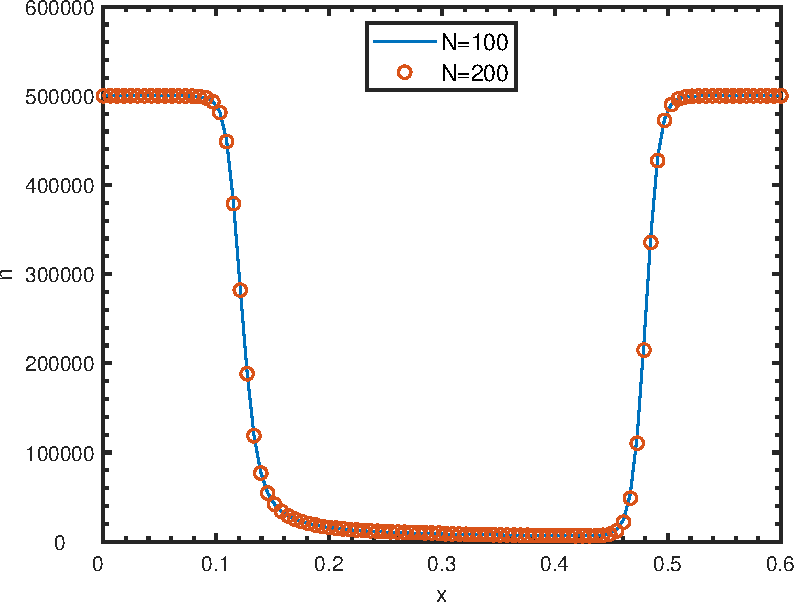
\includegraphics[width=\linewidth]{figure/DDTVDRK3Degree2mu0.75Nn.pdf}
    \end{minipage}
    \begin{minipage}{0.48\textwidth}
        \centering
        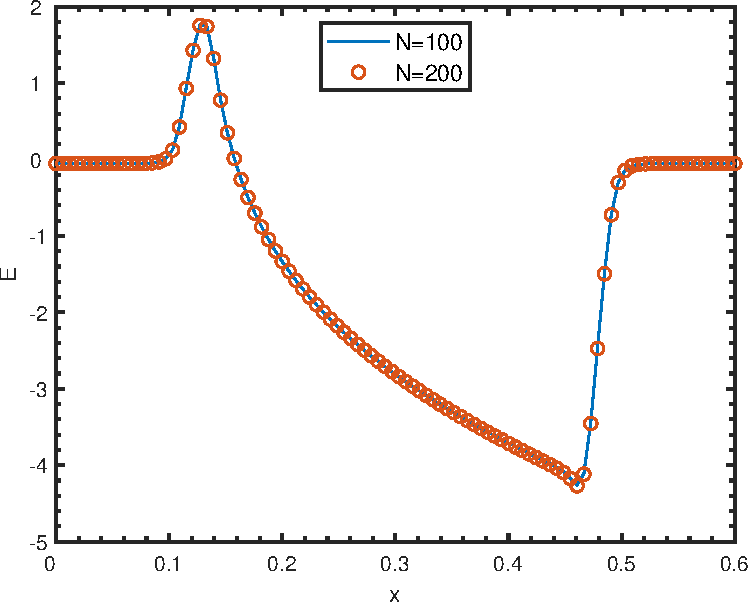
\includegraphics[width=\linewidth]{figure/DDTVDRK3Degree2mu0.75NE.pdf}
    \end{minipage}

    \centering
    \begin{minipage}{0.48\textwidth}
        \centering
        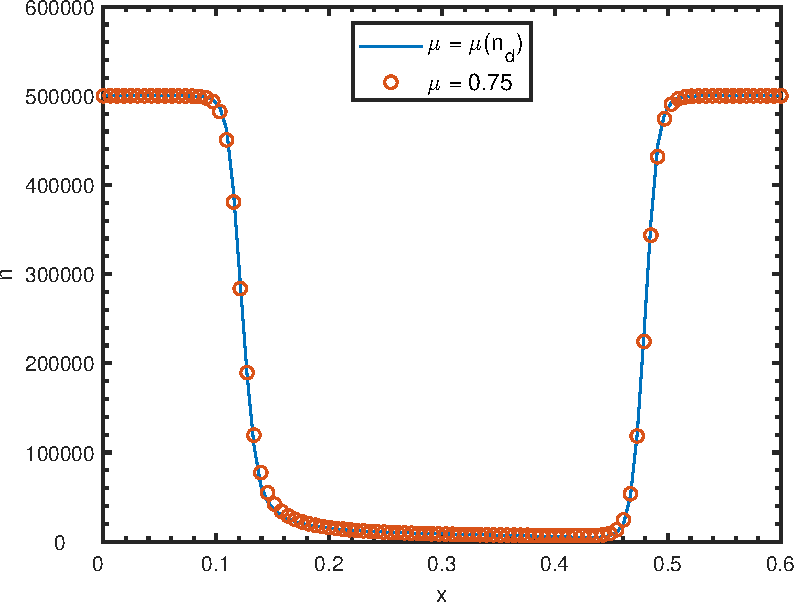
\includegraphics[width=\linewidth]{figure/DDTVDRK3Degree2N100mun.pdf}
    \end{minipage}
    \begin{minipage}{0.48\textwidth}
        \centering
        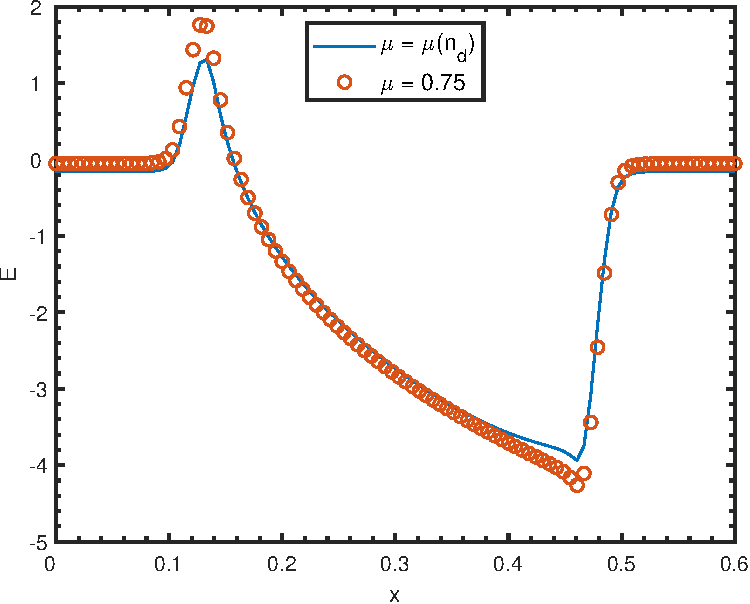
\includegraphics[width=\linewidth]{figure/DDTVDRK3Degree2N100muE.pdf}
    \end{minipage}

    \centering
    \begin{minipage}{0.48\textwidth}
        \centering
        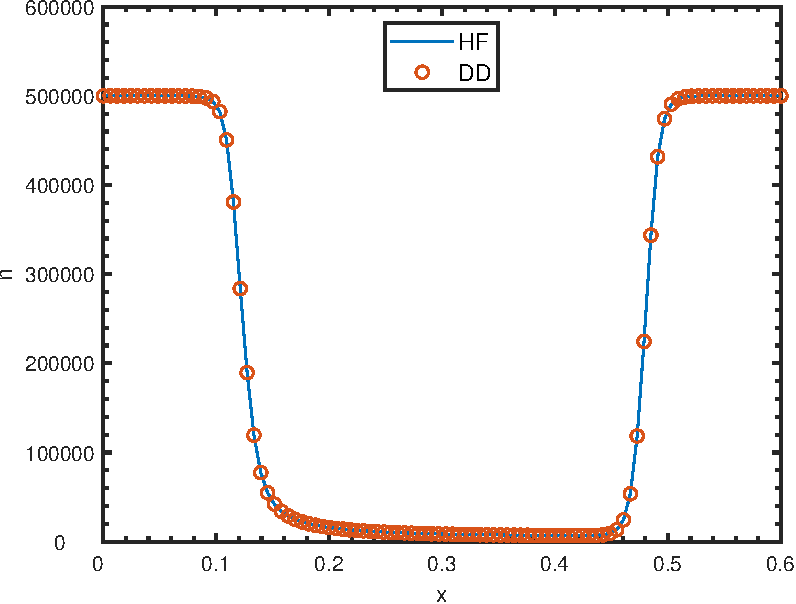
\includegraphics[width=\linewidth]{figure/DDTVDRK3Degree2N100mu0.75modeln.pdf}
    \end{minipage}
    \begin{minipage}{0.48\textwidth}
        \centering
        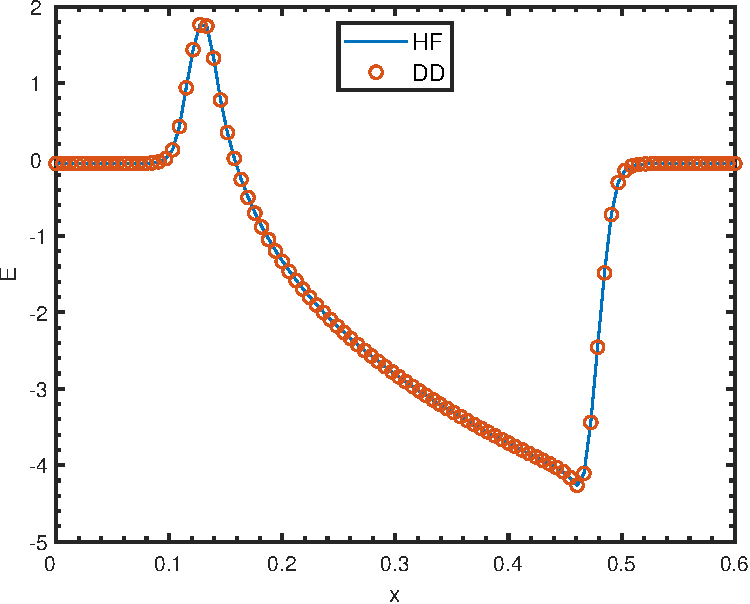
\includegraphics[width=\linewidth]{figure/DDTVDRK3Degree2N100mu0.75modelE.pdf}
    \end{minipage}
    \caption{默认值:DD模型三阶TVDRK,计算空间$V^2$,网格数$N=100$,迁移率$\mu=0.75$。左:电子浓度n;右:电势E。参数:上,网格数N;中,迁移率$\mu$;下,模型类型。}
    \label{fig:TVDRK}
\end{figure}

由于篇幅限制,这里只给出DD模型在网格数$N=100$和$N=200$情况下的全变差变化图,如\autoref{fig:TVDRKTV}所示,可以看到在一定误差范围内,总变差基本满足总变差不增。
\begin{figure}
    \centering
    \begin{minipage}{0.48\textwidth}
        \centering
        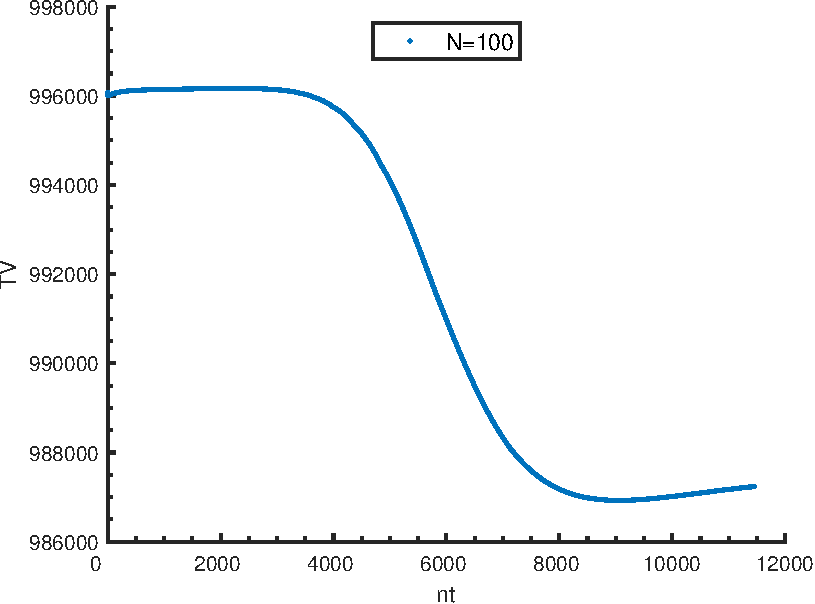
\includegraphics[width=\linewidth]{figure/TVDRKN100.pdf}
    \end{minipage}
    \begin{minipage}{0.48\textwidth}
        \centering
        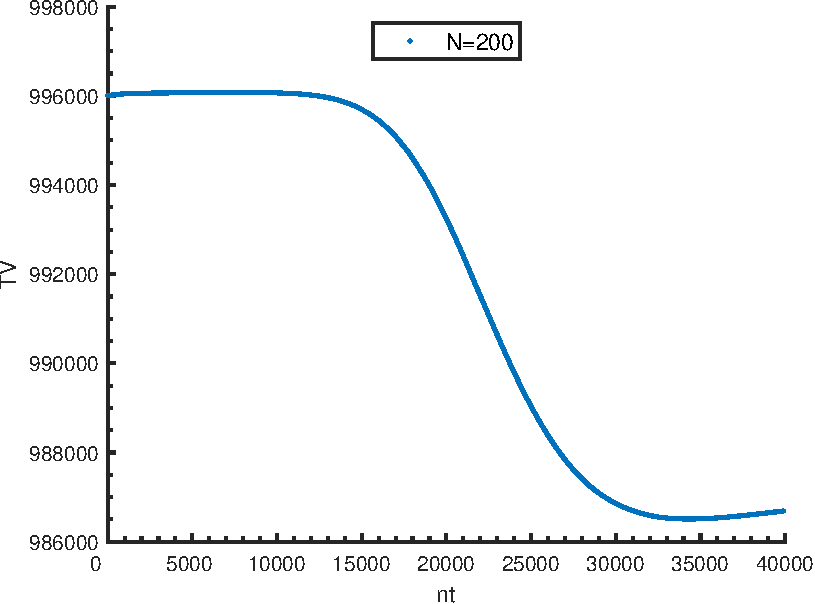
\includegraphics[width=\linewidth]{figure/TVDRKN200.pdf}
    \end{minipage}
    \caption{默认值:DD模型三阶TVDRK,计算空间$V^2$,网格数$N=100$和$N=200$,迁移率$\mu=0.75$。左:电子浓度n;右:电势E。}
    \label{fig:TVDRKTV}
\end{figure}

\autoref{fig:TVDRKLimiter}是添加了改进后的minmod限制器和无添加minmode限制器的图像,由于我们的解具有良好光滑性,同时计算空间选择为$V^2$,因此是否添加限制器基本上不会产生影响。
\begin{figure}
    \centering
    \begin{minipage}{0.48\textwidth}
        \centering
        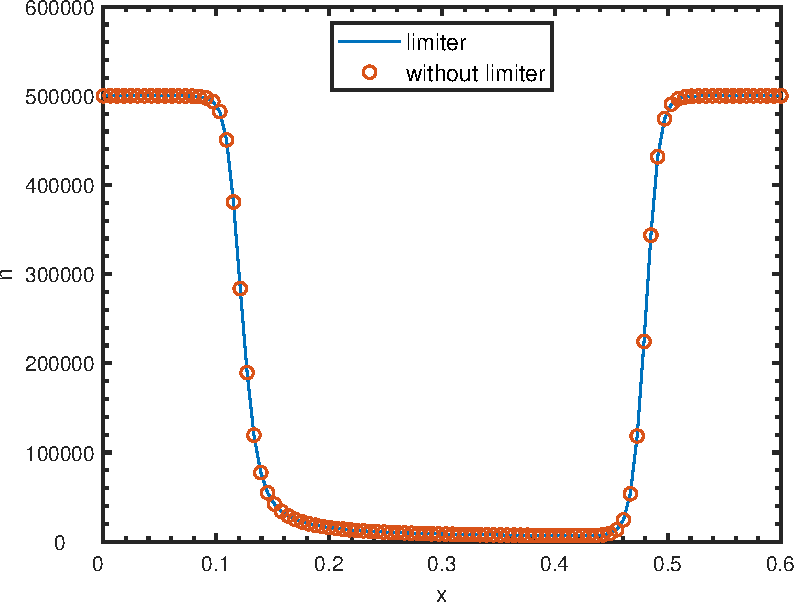
\includegraphics[width=\linewidth]{figure/DDTVDRK3Degree2N100mu0.75limitern.pdf}
    \end{minipage}
    \begin{minipage}{0.48\textwidth}
        \centering
        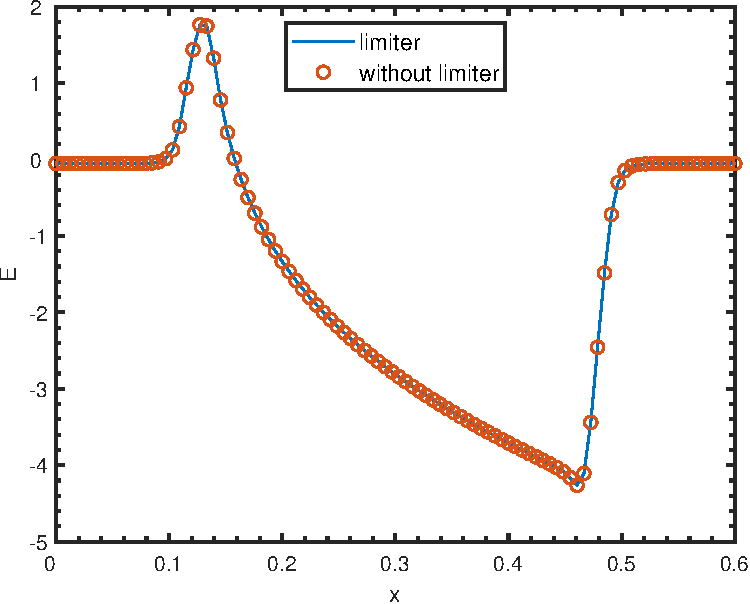
\includegraphics[width=\linewidth]{figure/DDTVDRK3Degree2N100mu0.75limiterE.pdf}
    \end{minipage}
    \caption{默认值:DD模型三阶TVDRK,计算空间$V^2$,网格数$N=100$,迁移率$\mu=0.75$。x:时间层;TV:全变差。}
    \label{fig:TVDRKLimiter}
\end{figure}
但如果我们的计算空间选择$V^k , k\geq 3$,如果直接让三次基函数项的系数直接取零,在数值模拟过程中仅在数个时间层后就出现了明显的误差。一般来讲,直接让三次项的系数保持不变即可,但考虑到本文模型假定了解具有良好的光滑性,又构造出了足够光滑的初始函数,不需要限制器也可以正确模拟。因此对于限制器更深入的讨论,可以在未来分析具有强震荡解的模型时再详细研究。

\subsection{IMEX LDG格式}
由于没有准确解的显式表达式,我们采取细网格上的数值解来代替真实解。
我们取网格数$N=3200$计算空间$V_h^2$的数值解作为真实解,我们有\autoref{tab:IMEXLDGerror}的误差估计
\begin{table}
    \begin{tabular}{ccc}
        \toprule
            & \multicolumn{2}{c}{$V^0$}               \\
        \cmidrule{2-3}
        N   & $\frac{||u_h-u||}{||u||}$ & order       \\

        \midrule
        25  & 9.94e-02                  & \text{----} \\
        50  & 5.50e-02                  & 0.85        \\
        100 & 2.80e-02                  & 0.97        \\
        200 & 1.43e-02                  & 0.97        \\
        400 & 7.07e-03                  & 1.02        \\
        800 & 3.44e-03                  & 1.04        \\
        \bottomrule
    \end{tabular}
    \caption{IMEX LDG格式误差估计}
    \label{tab:IMEXLDGerror}
\end{table}

